\section{Evaluation and Performance}
\label{sec:eval}

We evaluated CommunityGuard by both the effectiveness of its intended operation~\ref{sec:eval:operation} as well as by network performance while the system was running in-line ~\ref{sec:eval:performance}.  


\subsection{Operation}
\label{sec:eval:operation}

To test the effectiveness of the system, we evaluated two core capabilities of CommunityGuard which are described below.
Our \textit{Test Setup} includes two Guardian Nodes (in this case two configured BeagleBone Black devices each between a modem and router) present on different networks, which were used to test the system to check if blacklisted IP addresses updated by one Guardian Node  was communicated to the other. Both Guardian Nodes connected to the Community Outpost server with the same periodicity.

%\begin{figure}
%    \centering
%    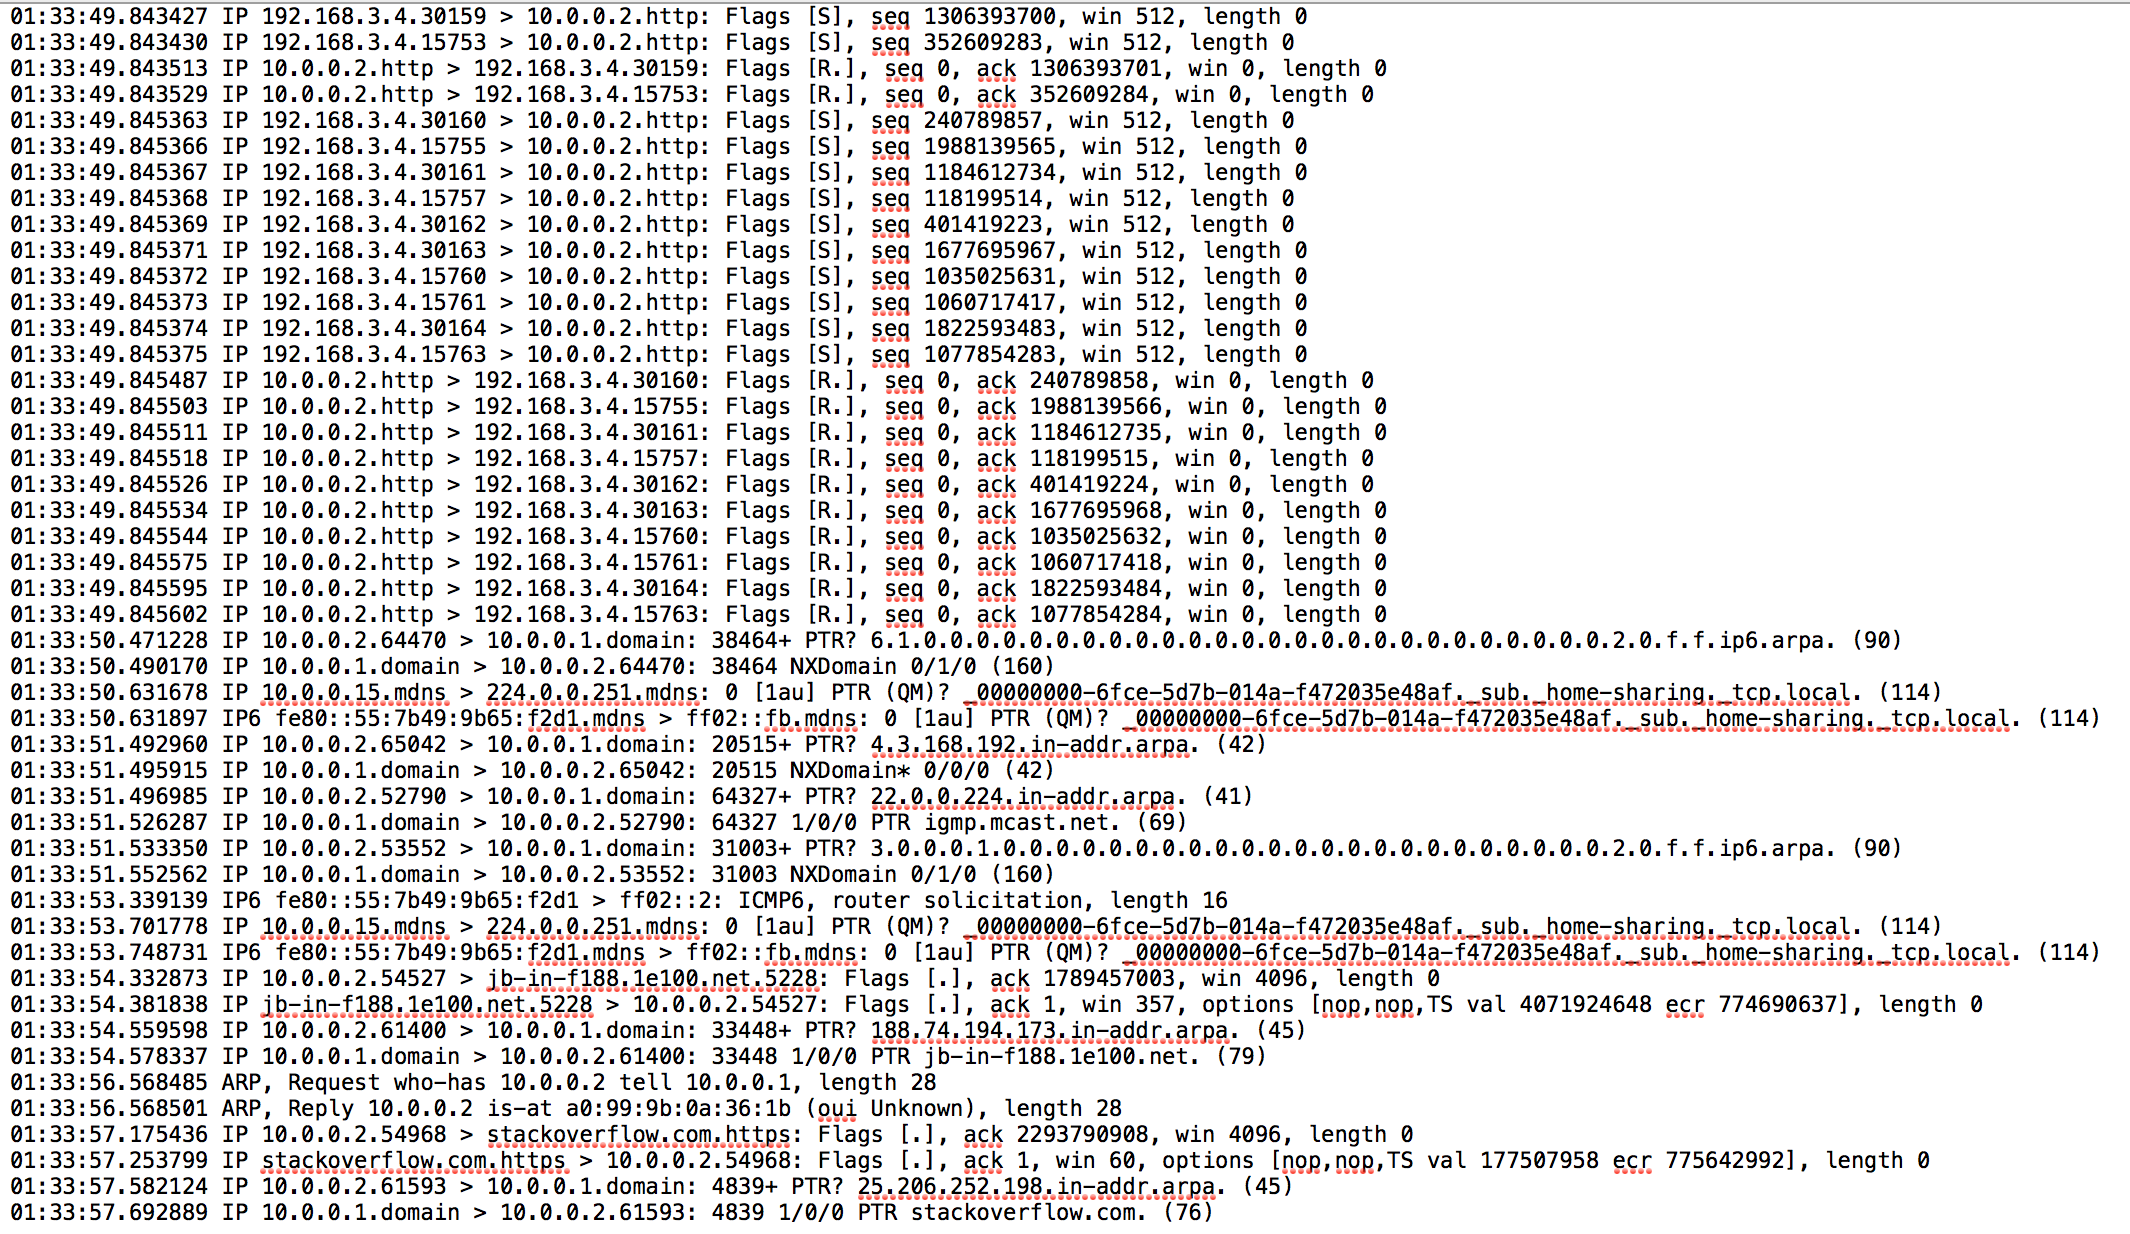
\includegraphics[width=0.95\linewidth, height=4cm]{figs/tcpdump.png}
%    \caption{TCP dump at DDoS target}
%    \label{fig:tcpdump}
%\end{figure}
\subsubsection{Prevent and log incoming malicious traffic}
\label{sec:eval:preventout}

 Snort rules were configured to block IP traffic that contained malicious content. There are thousands of open-source snort rules available that can alert and drop malicious traffic like worms, illegal attempts at accessing FTP or telnet, and a range of attacks ~\cite{Roesch:1999:SLI:1039834.1039864}. However, we did not wish to receive actual malicious traffic in testing due to infrastructure and resource restrictions. Instead, the team wrote a few snort rules to treat some arbitrary safe traffic as malicious and configured rules to drop such traffic. 
%Figure~\ref{fig:snortrule} shows a screenshot of a sample Snort rule that alerts and logs all traffic containing the word "cat". Figure~\ref{fig:snortrule} also shows a section of the log where the "malicious" traffic was spotted. 
The cron job (discussed in \ref{sec:design:software}) parsed the log and updated the DB about the source from where possible malicious traffic was originating. Depending on a majority of votes (this majority was artificially elevated in our test case since only two Guardian Nodes were present), the Community Outpost proceeded to conditionally add the malicious source IP to the blocked list. Newly confirmed bad IP addresses are fetched when the cron job responsible for adding blacklisted IP addresses next runs on the Guardian Nodes. %In case of the log shown in Figure \ref{fig:snortrule}, IP addresses "107.23.60.9" and "72.21.91.66" were treated as Bad IPs, and were subsequently blocked by both Guardian Nodes once the cron job refreshed the blacklist with the latest one from the Community Outpost.

\subsubsection{Prevent outbound DDoS attacks}
\label{sec:eval:outddos}

This was tested by adding "fake" DDoSed IP addresses to the DDoS watch list on the Community Outpost. The DDoSed IP addresses were friend machines in another network. In a real world implementation, we assume that a Third Party DDoS protection service \cite{DDoSPreventionTools} that has been specifically employed for the job would update the DDoSed IP addresses to the CommunityGuard administrators. The team added the DDoSed IP addresses manually in order to test this functionality. A TCP SYN DoS attack was simulated with hping3 \cite{hpingReferralPaper} \cite{hping}.  The cron job that was checking for new updates from the database fetched these IP addresses every minute and checked for a match in the existing list of DDoSed IP addresses maintained at each Guardian Node. New Snort drop rules were created for these IP addresses if a match was not found. The new rules prevent all outbound DDoS traffic to the IP addresses fetched from the DDoS watch list. 

An important point to note here is that the network was still allowed to send legitimate traffic to these attacked IP addresses because Snort rules were configured to monitor the pattern of a DDoS attack before dropping that traffic. One such Snort rule is shown in Figure ~\ref{fig:snortrule1} which detects an outgoing SYN flood attack from the home network to an external network. Figure ~\ref{fig:snortrule1} also shows the log created by Snort when it detects and drops an outgoing DDoS attack as soon as the cron job fetches the DDoS watch list from the Community Outpost. The Snort rule detects TCP-SYN DDoS attack patterns and drops all such outgoing traffic. However, benign TCP traffic is still allowed to pass through. This was tested using the netcat tool \cite{netcat} to communicate between the attacking system and the attacked system via TCP while Snort was actively blocking all outgoing TCP-SYN DDoS attacks to the target IP.

\subsection{Performance}
\label{sec:eval:performance}
\subsubsection{Load test}
\label{sec:eval:loadtest}
The Guardian Node is designed to be inserted in-line somewhere before the Router, which implies that the Guardian Node could be introducing a possible bottleneck and stalling traffic coming into and going out of the personal network. Therefore, it was necessary to verify the performance of the Guardian Node while it was fully functional. Speed tests were taken at intervals of 5 minutes under light, average and heavy load conditions to conform performance compliance. Light load was simulated by opening 1-3 video Live streams, a few browsers with medium flash content, one active upload and few Social media pages over 6 different devices ranging from desktops to tablets and mobile phones. Average load was simulated by opening 3-5 live streams, 4-6 pages with high flash content and 2-3 active uploads distributed over the same set of devices. Heavy load was simulated by increasing to 6-8 live streams, 8-10 pages with high flash content and 4-5 active uploads distributed over the same set of devices. Figure ~\ref{fig:graph} shows the performance represented as a linear plot. As can be seen, the performance data is very similar between the baseline and the test case. On an average the test case appears to be slightly lower than the baseline case which can be significantly attributed to the following hardware deficiencies.
\begin{itemize}
    \item USB to 10/100 Mbps Ethernet adapter --
    The Guardian Node hardware, which in this case was a BeagleBone Black, has only one on-board 10/100 Mbps Ethernet port. An USB to 10/100 Mbps Ethernet adapter was added since the Guardian Node required two network interfaces. Speed of transfer was therefore severely limited by the speed of conversion.
    \item Slow SD card writes --
    The Guardian Node was running a Linux Operating System that was mounted on a SD card. Transfer speeds were also affected by comparatively slow SD card write times.
\end{itemize}

%\begin{figure}
%    \centering
%    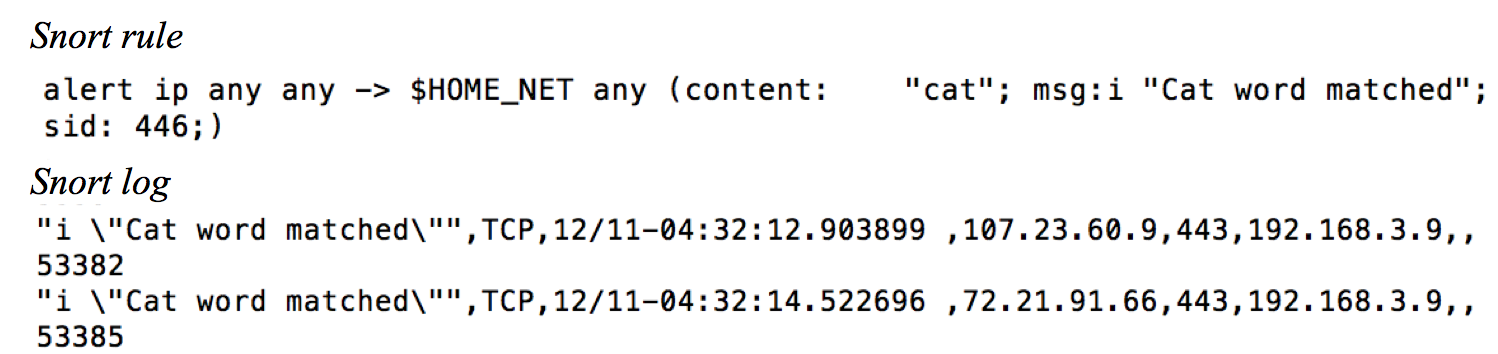
\includegraphics[width=0.95\linewidth]{figs/catrule.png}
%    \caption{Sample Snort rule and log}
%    \label{fig:snortrule}
%\end{figure}

\begin{figure}
	\centering
%	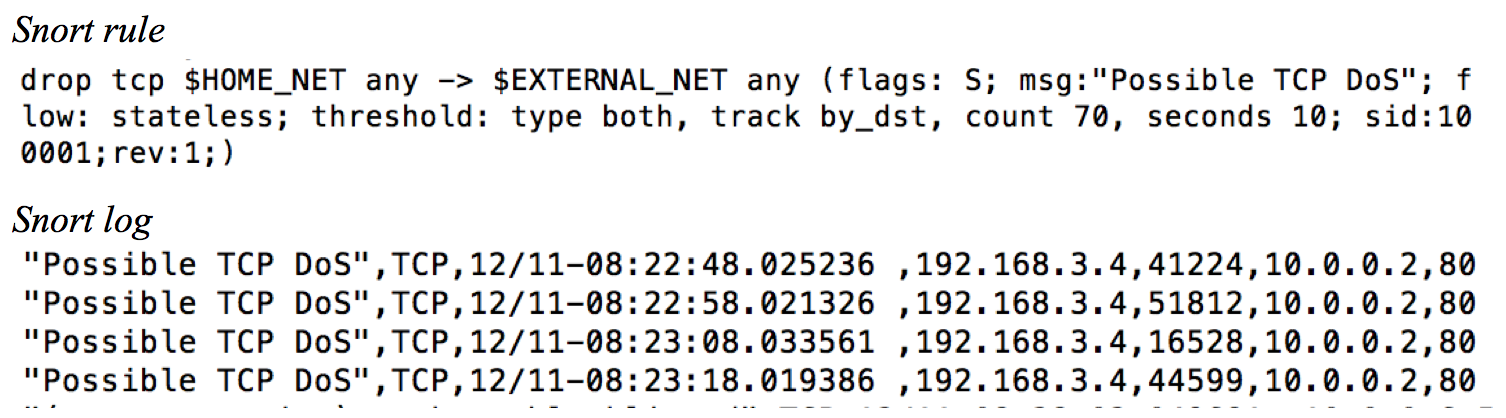
\includegraphics[ height=2.2cm]{figs/ddosrule.png}
	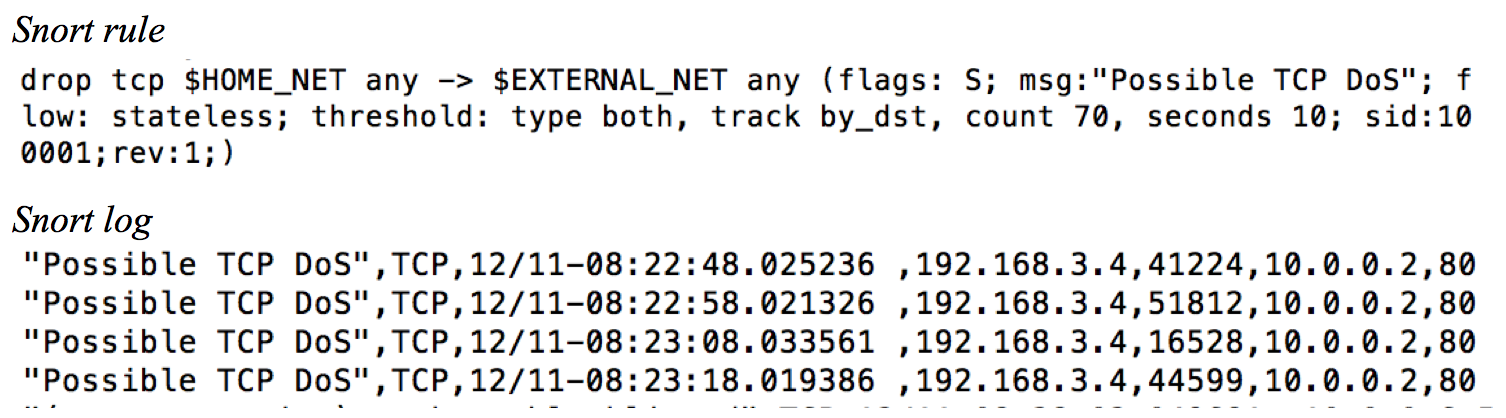
\includegraphics[width=\columnwidth]{figs/ddosrule.png}
	\caption{Sample Snort DDoS prevention rule and log}
	\label{fig:snortrule1}
\end{figure}

\begin{figure*}
	\centering
%	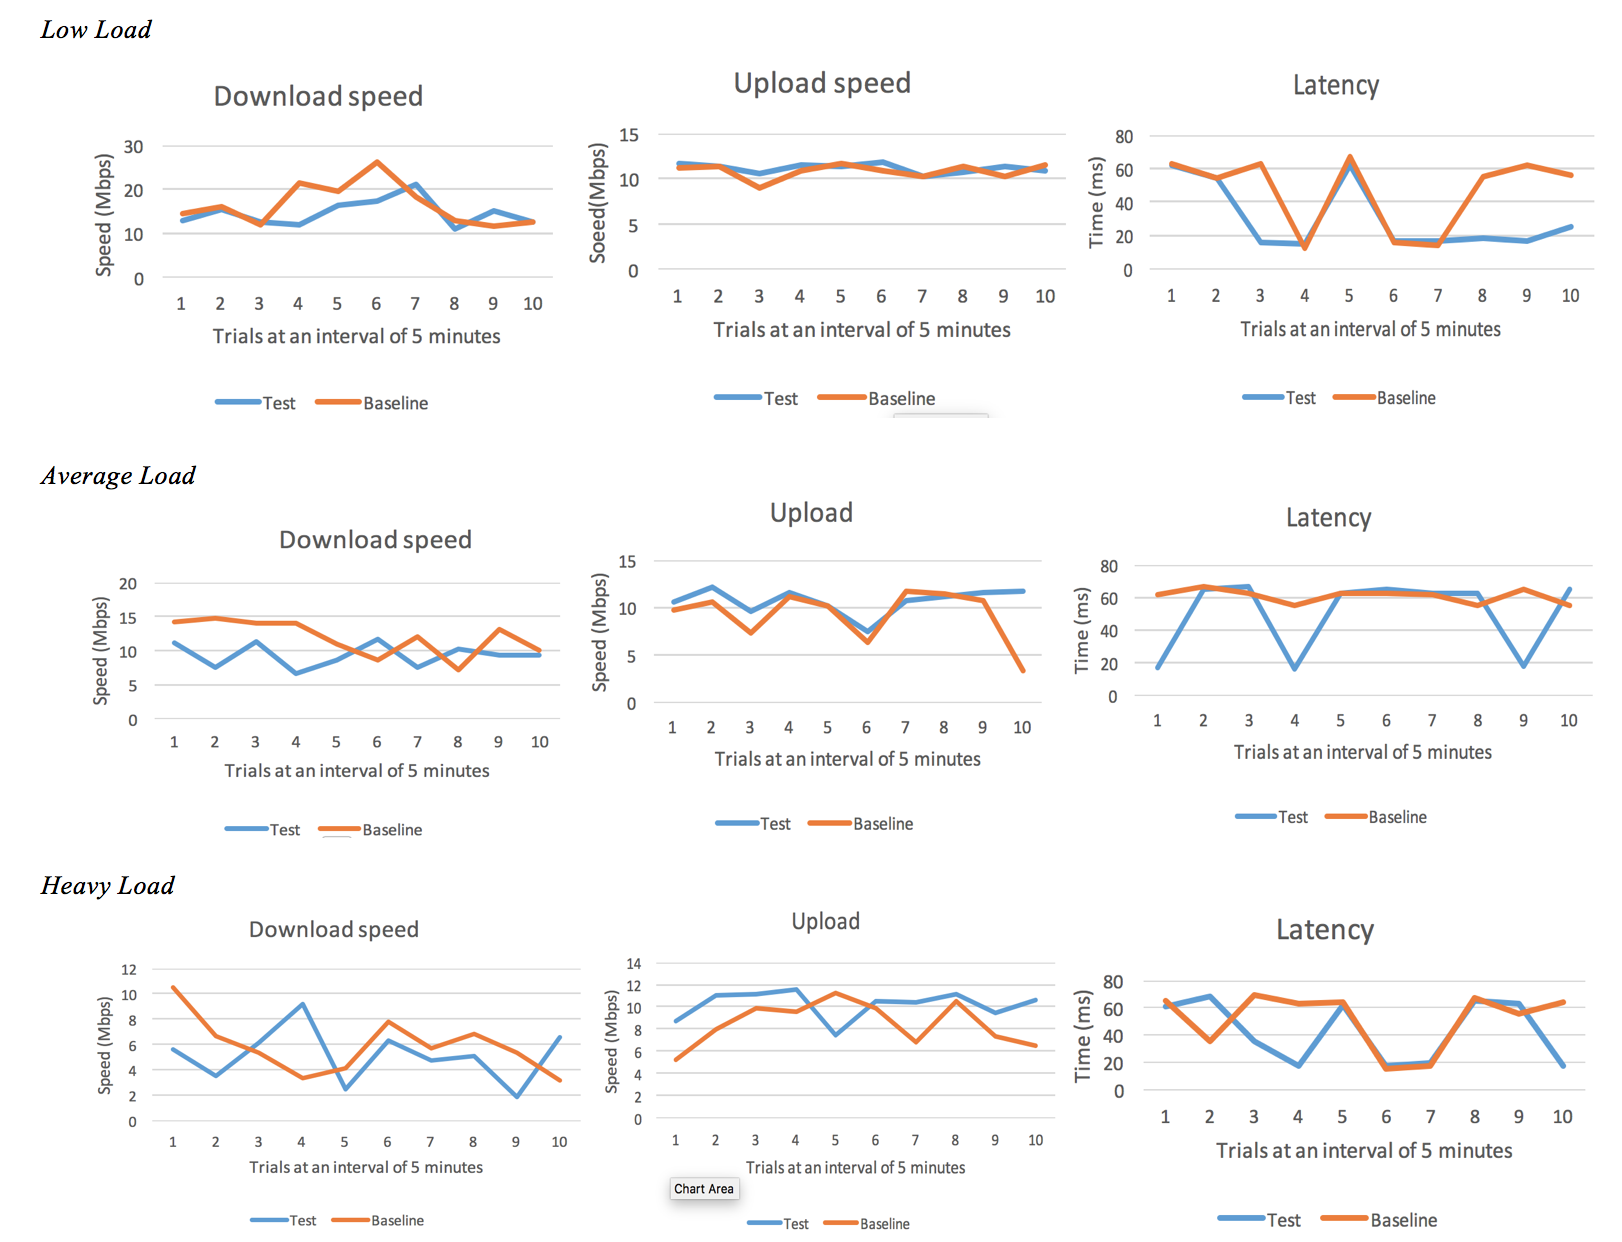
\includegraphics[width=0.7\linewidth, height=5.5cm]{figs/graph.png}
	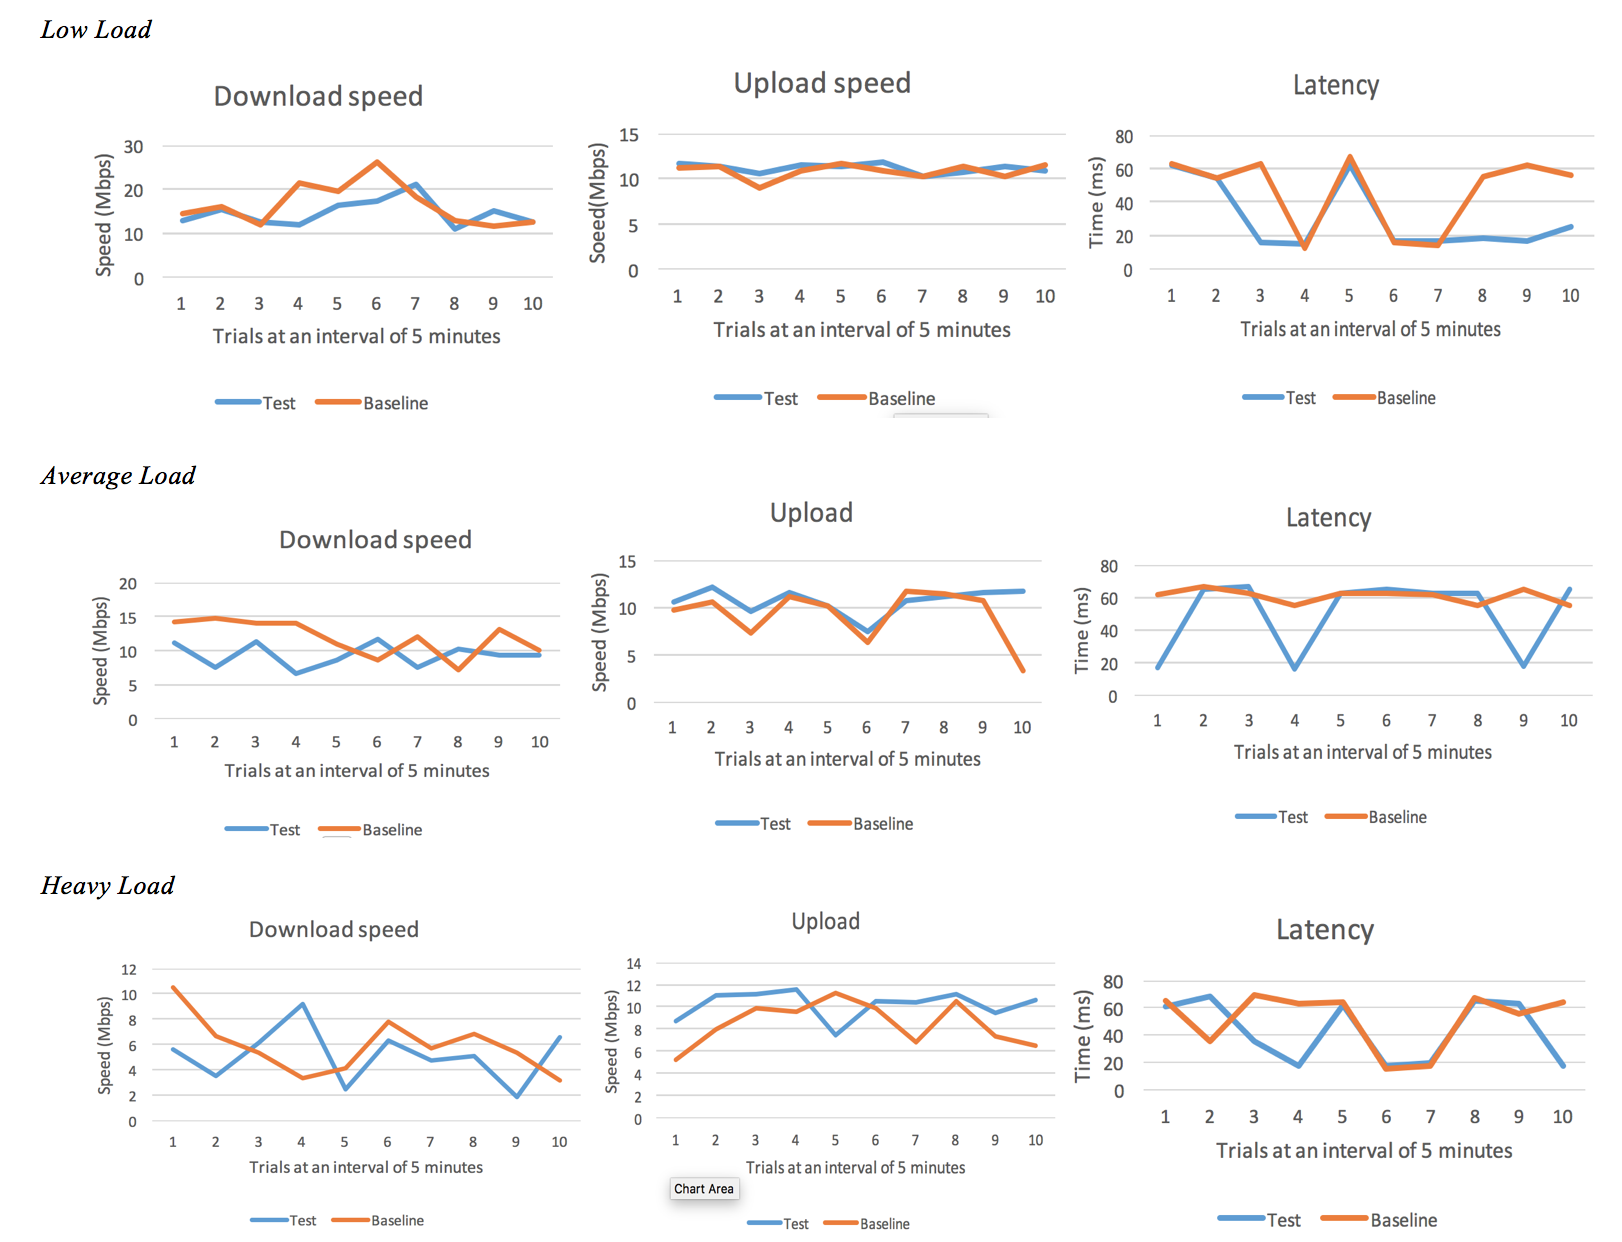
\includegraphics[width=0.75\linewidth]{figs/graph.png}
	\caption{Results of Snort throughput tests: test=CommunityGuard, baseline=no CommunityGuard}
	\label{fig:graph}
\end{figure*}

\subsubsection{Performance vs. number of Snort rules}
\label{}
Snort provides the freedom to configure as few rules or as many rules as required. The Load Test mentioned in Section \ref{sec:eval:loadtest} was done with approximately 7000 Snort rules configured and functioning. Speed tests were also conducted for a number of rules ranging between 100 to 10000. It was seen that the number of rules did not affect speed test results as much as one would expect. Speed measurements indicated similar values to those shown in Figure ~\ref{fig:graph}. This was attributed to the fact that Snort processes utilized around 150 to 200 MB of RAM in all cases ranging between 100 to 10000 rules. Figure ~\ref{fig:ramutil} shows the RAM utilization without Snort running, Snort running with 156 rules and Snort running with 9863 rules. 

The CommunityGuard team  feels that the set of running Snort rules can be further optimized for better processor and RAM utilization. Optimization of Snort rules will be pursued as future work. It is to be noted that increasing traffic from 100 Mbps to 400 Mbps will increase the RAM requirement to almost 1GB for 100-10000 rules. The implementation of Snort on the Guardian Node was using much less RAM since network traffic was limited to 100 Mbps by the Ethernet card. Dealing with higher traffic speeds would require specialized hardware. In an ideal implementation, the Guardian Node would have a network card with performance specifications equivalent to it's router's network card.

\begin{figure}
    \centering
%    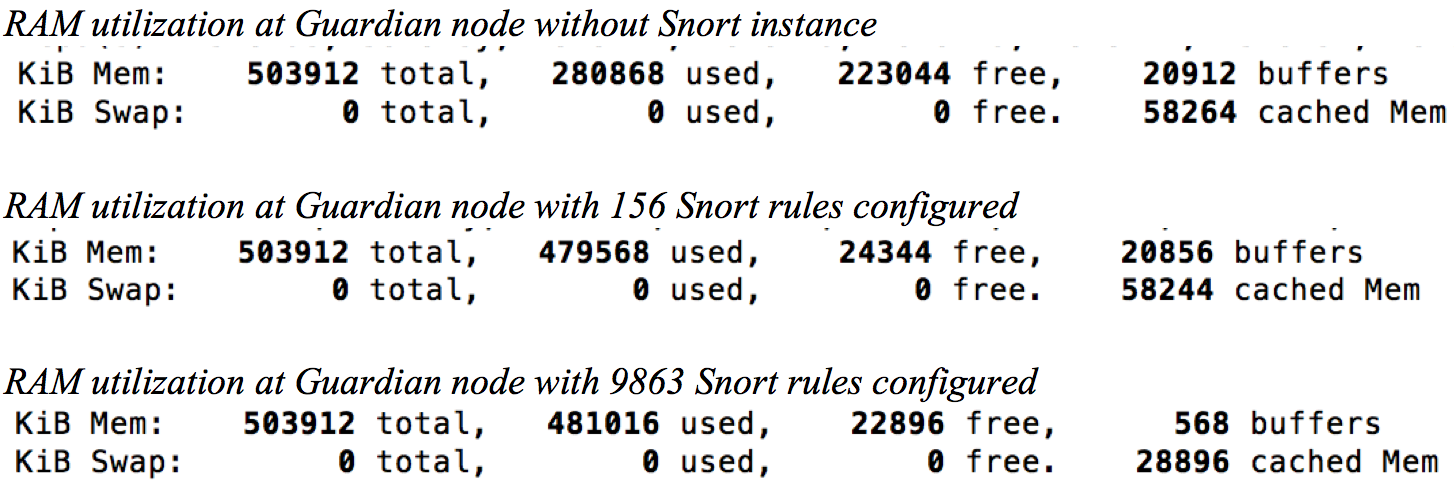
\includegraphics[width=0.85\linewidth,  height=2cm]{figs/SnortRam.png}
    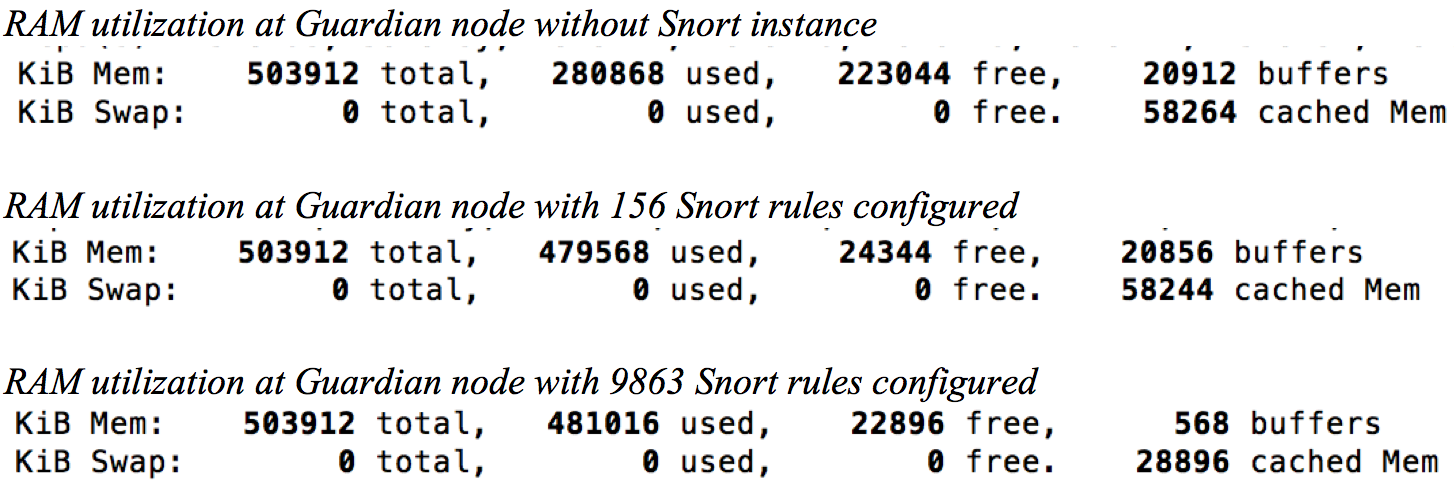
\includegraphics[width=0.85\columnwidth]{figs/SnortRam.png}
    \caption{RAM Utilization on the Guardian Node}
    \label{fig:ramutil}
\end{figure}

